%%%%%%%%%%%%%%%%%%%%%%%%%%%%%%%%%%%%%%%%%%%%%%%%%%%%%%%%%%%%%%%%%%%%%%%%%%%%%%%%%%%%%%%
%%%%%%%%%%%%%%%%%%%%%%%%%%%%%%%%%%%%%%%%%%%%%%%%%%%%%%%%%%%%%%%%%%%%%%%%%%%%%%%%%%%%%%%
%%%%%%%%%%%%%%%%%%%%%%%%%%%%%%%%%%%%%%%%%%%%%%%%%%%%%%%%%%%%%%%%%%%%%%%%%%%%%%%%%%%%%%%
\section{Minimização de $||h(x)-a||^2+\alpha ||x-b||^2$}

%\index{Problema inverso!Não linear}
\index{Minimização do erro quadrático!Não linear}%!Função $||h(x)-a||^2+\alpha ||x-b||^2$}

\begin{theorem}[Solução iterativa:]\label{theo:minhxhxxbxb}
Dados
um escalar $\alpha \in \mathbb{R}_+$, 
um escalar $x \in \mathbb{R}$, 
um escalar $a \in \mathbb{R}$,  
uma função $h:\mathbb{R} \rightarrow \mathbb{R}$, e 
definida a Eq. (\ref{eq:minhxhxxbxb1}),
\begin{equation}\label{eq:minhxhxxbxb1}
e(x)=||h(x)-a||^2+\alpha ||x-b||^2.
\end{equation}
Se desejarmos ter o valor $x=\hat{x}$ que minimiza o escalar $e(x)$,
esse valor pode ser achado\footnote{A 
demonstração da Eq (\ref{eq:minhxhxxbxb2}) pode ser vista na Prova \ref{proof:theo:minhxhxxbxb}.} 
 usando iterativamente a Eq. (\ref{eq:minhxhxxbxb2}),
em que $h'(x)\equiv \frac{d h(x)}{d x}$,
\begin{equation}\label{eq:minhxhxxbxb2}
x_{k} \leftarrow x_{k-1}-
\frac{ h'(x_{k-1}) \left[h(x_{k-1})-a\right]+\alpha\left[ x_{k-1}-b\right]}{\left[h'(x_{k-1})\right]^2+\alpha}.
\end{equation}
Assim, $\hat{x}$ pode ser achado iniciando a Eq. (\ref{eq:minhxhxxbxb2}) desde um 
$x_{0}$ qualquer, realizando cálculos $x_{k}$ iterativamente, 
até que $x_{k}$ seja muito próximo a $x_{k-1}$ (convergência de $x_{k}$); assim,
baixo essas condições declaramos que $\hat{x} \approx x_{k}$.

\textbf{Considerações:}
\begin{itemize}
\item É interessante verificar na Eq. (\ref{eq:minhxhxxbxb2}) 
se  $h'(x_{k-1}=b) = 0$,
pois indica que existe um ponto de inflexão 
(máximo, mínimo ou ponto de sela) em $e(x_{k-1}=b)$;
consequentemente poderiamos ter achado um mínimo\footnote{É 
interesante verificar o ponto $b$, uma vez só, 
antes de iniciar a busca iterativa.}.
\end{itemize}

\end{theorem}

\begin{tcbattention}
\begin{itemize}
\item O Teorema \ref{theo:minhxhxxbxb} pode ser usado para achar o ponto $x$
que minimize $e(x)=||h(x)-a||^2+\alpha||x-b||^2$,
quando sabemos que o vetor $x$ que minimiza $||h(x)-a||^2$ 
está perto do ponto $b$.
\item No Teorema \ref{theo:minhxhxxbxb}, o ponto $x$ que minimiza $e(x)$ 
não necesariamente minimiza  $||h(x)-a||^2$.
\end{itemize}
\end{tcbattention}


%%%%%%%%%%%%%%%%%%%%%%%%%%%%%%%%%%%%%%%%%%%%%%%%%%%%%%%%%%%%%%%%%%%%%%%%%%%%%%%%
\subsection{Exemplos de minimização de $||h(x)-a||^2+\alpha ||x-b||^2$}


\begin{example}\label{ex:minhxhxxbxb1}
Conhecida uma função $h(x)=x^2(x^2-1)$, o valor $a=1$ do contradomínio de $h(x)$,
o fator $\alpha=1.2$ e o ponto $b=0$,
achar o valor $x=\hat{x}$ que minimize $e(x)=||h(x)-a||^2+\alpha||x-b||^2$.
\end{example}
\begin{SolutionT}[Relativa ao Exemplo \ref{ex:minhxhxxbxb1}:]\label{sol:minhxhxxbxb1}


 A Fig. \ref{fig:hxbcasesa} nos mostra o processo de busca de um mínimo
 de $e(x)$. A busca inicia em $x_0=-1.4$,
 todos os valores $x_{k}$ podem ser vistos na Tabela \ref{tab:hxbcases1}. 
Neste caso, a busca iterativa indicada pela Eq. (\ref{eq:minhxhxxbxb2}) converge sem problemas 
em $\hat{x}\approx x_7 =-1.21239$ com $e(x_7)=1.85954$; porém, 
 este valor de $x$ é um mínimo local e está longe do mínimo
 global de  $e(x)$ que está em $x=0$ com um $e(0)=1.0$.
\begin{comment}
 $x_7$ é um mínimo local de $e(x)$
 e está perto do mínimo global $x=\pm\sqrt{\frac{1+\sqrt{5}}{2}}\approx \pm1.2720$ 
de  $||h(x)-a||^2$; esta diferença é consequência do uso do fator 
 $\alpha>0$, pelo qual é de esperar que quanto maior seja o valor de $\alpha$
 maior será a diferencia da posição do mínimo global de $e(x)$ e de $||h(x)-a||^2$.
\end{comment}
\end{SolutionT}



\begin{table}[!h]
\centering
\begin{tabular}{|l|l|l|l|l|l|l|l|l|}
\hline
$k$      & 0 & 1 & 2 & 3 & 4 & 5 & 6 & 7 \\ \hline
$x_k$    & -1.4000 & -1.2694 & -1.2258 & -1.2153 & -1.2130 & -1.2125 & -1.2124 & -1.2124 \\ \hline
$e(x_k)$ & 3.1292 & 1.9338 & 1.8631 & 1.8597 & 1.8595 & 1.8595 & 1.8595 & 1.8595 \\ \hline
\end{tabular}
\caption{Resposta iterativa do Exemplo \ref{ex:minhxhxxbxb1}.}
\label{tab:hxbcases1}
\end{table}

\begin{figure}[!h]
    \centering
    \begin{subfigure}[b]{0.49\textwidth}
        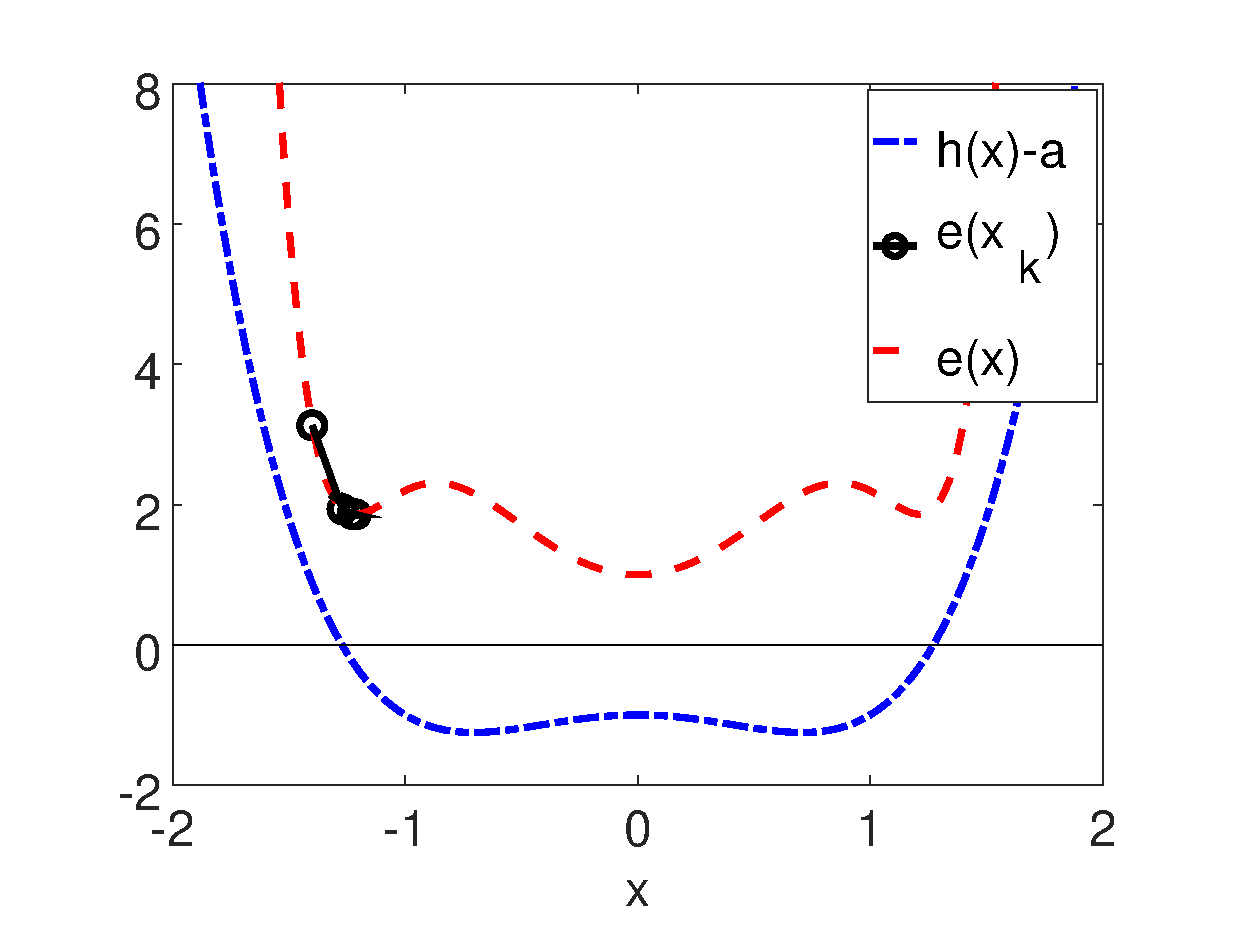
\includegraphics[width=\textwidth]{chapters/minimization-hx/mfiles/hx_a_alphax/minimizando_hx_a_alphax_1.eps}
        \caption{Usando $h(x)=x^2(x^2-1)$, $a=1$, $b=0$ e $\alpha=1.2$, quando as iterações convergem.}
        \label{fig:hxbcasesa}
    \end{subfigure}
    ~ %add desired spacing between images, e. g. ~, \quad, \qquad, \hfill etc. 
      %(or a blank line to force the subfigure onto a new line)
    \begin{subfigure}[b]{0.49\textwidth}
        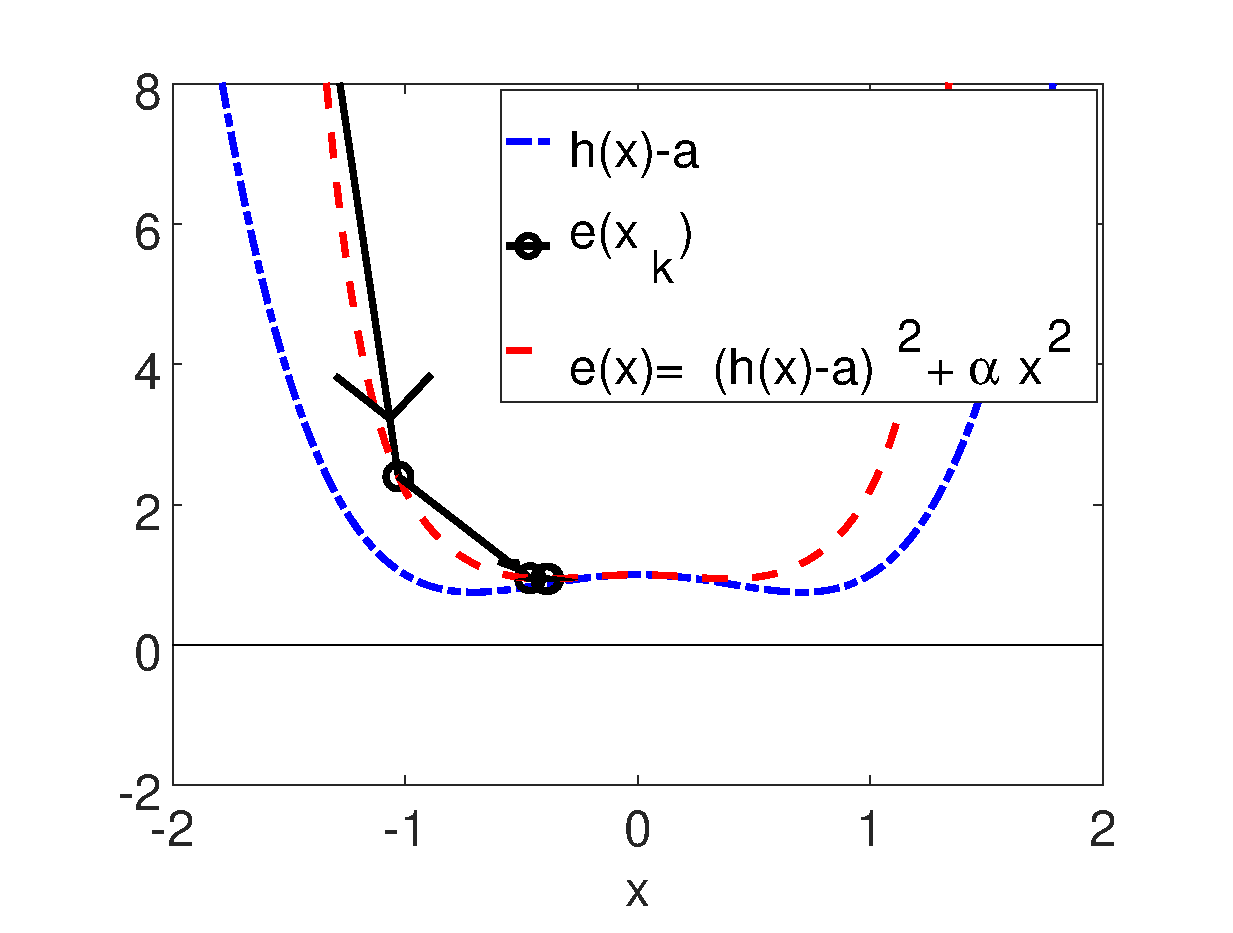
\includegraphics[width=\textwidth]{chapters/minimization-hx/mfiles/hx_a_alphax/minimizando_hx_a_alphax_2.eps}
        \caption{Usando $h(x)=x^2(x^2-1)$, $a=-1$, $b=0$ e $\alpha=1.2$, quando as iterações convergem.}
        \label{fig:hxbcasesb}
    \end{subfigure}
    \caption{Comportamento para $h(x)=x^2(x^2-1)$ da equação iterativa do Teorema \ref{theo:minhxhxxbxb}.}
    \label{fig:hxbcases}
\end{figure}


\begin{example}\label{ex:minhxhxxbxb2}
Conhecida uma função $h(x)=x^2(x^2-1)$, o valor $a=-1$ que não existe no contradomínio de $h(x)$,
o fator $\alpha=1.2$ e o ponto $b=0$,
achar o valor $x=\hat{x}$ que minimize $e(x)=||h(x)-a||^2+\alpha||x-b||^2$.
\end{example}
\begin{SolutionT}[Relativa ao Exemplo \ref{ex:minhxhxxbxb2}:]\label{sol:minhxhxxbxb2}
 A Fig. \ref{fig:hxbcasesb} nos mostra o processo de busca de um mínimo
 de $e(x)$. A busca inicia em $x_0=-1.4$,
 todos os valores $x_{k}$ podem ser vistos na 
Tabela \ref{tab:hxbcases2}. Neste caso, a busca iterativa indicada pela Eq. (\ref{eq:minhxhxxbxb2}) converge
em $\hat{x}\approx x_7=-0.39349$ com $e(\hat{x})=0.94120$, que é um mínimo global de $e(x)$.
\begin{comment}
; porém, este valor de $x_k$ está
um pouco distante do mínimo de $(h(x)-a)^2$, localizado em $x=\pm\frac{\sqrt{2}}{2}\approxeq \pm0.70711$.
Novamente, isto é consequência do uso do fator 
 $\alpha>0$, assim, quanto maior seja o valor de $\alpha$
 maior será a diferencia do mínimo global de $e(x)$ e de $(h(x)-a)^2$.
\end{comment}
\end{SolutionT}

\begin{table}[!h]
\centering
\begin{tabular}{|l|l|l|l|l|l|l|l|l|}
\hline
$k$      & 0 & 1 & 2 & 3 & 4 & 5 & 6 & 7 \\ \hline
$x_k$    & -1.4000 & -1.0290 & -0.4625 & -0.3849 & -0.3926 & -0.3934 & -0.3935 & -0.3935 \\ \hline
$e(x_k)$ & 10.65562 &  2.39969 &  0.94867 &  0.94130 &  0.94121 &  0.94120 &  0.94120 &  0.94120 \\ \hline
\end{tabular}
\caption{Resposta iterativa do Exemplo \ref{ex:minhxhxxbxb2}.}
\label{tab:hxbcases2}
\end{table}


\begin{example}\label{ex:minhx3hx3xbxb3}
Conhecida uma função $h(x)=(x+0.5)^3$, o valor $a=1$ no contradomínio de $h(x)$,
o fator $\alpha=0.01$ e o ponto $b=0$,
achar o valor $x=\hat{x}$ que minimize $e(x)=||h(x)-a||^2+\alpha||x-b||^2$.
\end{example}
\begin{SolutionT}[Relativa ao Exemplo \ref{ex:minhx3hx3xbxb3}:]\label{sol:minhx3hx3xbxb3}
 A Fig. \ref{fig:hx3bcasesa} nos mostra o processo de busca de um mínimo
 de $e(x)$. 
 A busca inicia em $x_0=-1.4$,
 todos os valores $x_{k}$ podem ser vistos na Tabela \ref{tab:hx3bcases3}. 
Neste caso, a busca iterativa indicada pela Eq. (\ref{eq:minhxhxxbxb2}) diverge
em $x_2$; após este evento as iterações continuam e convergem sem problemas 
em $\hat{x}\approx x_7=+0.53255$ com $e(\hat{x})\approx 0.013$.
\begin{comment}
; este valor de $x$ está perto do mínimo global de  $(h(x)-a)^2$, que está em  $x=+0.5$. 
Isto é consequência do uso do fator 
 $\alpha>0$ e pequeno, pelo qual é de esperar que quanto maior seja o valor de $\alpha$
 maior será a diferencia do mínimo global de $e(x)$ e de $(h(x)-a)^2$.
\end{comment}
\end{SolutionT}

\begin{table}[!h]
\centering
\begin{tabular}{|l|l|l|l|l|l|l|l|l|}
\hline
$k$      & 0 & 1 & 2 & 3 & 4 & 5 & 6 & 7 \\ \hline
$x_k$    & -1.400 & -0.68731 & 4.66500 & 2.95583 & 1.83178 & 1.11578 & 0.70475   & 0.53255 \\ \hline
$e(x_k)$ & 3.009 & 1.0179 & 1.8711e+4 & 1621.9 & 136.42 & 10.371 & 0.56538 & 0.013 \\ \hline
\end{tabular}
\caption{Resposta iterativa do Exemplo \ref{ex:minhx3hx3xbxb3}.}
\label{tab:hx3bcases3}
\end{table}

\begin{figure}[!h]
    \centering
    \begin{subfigure}[b]{0.49\textwidth}
        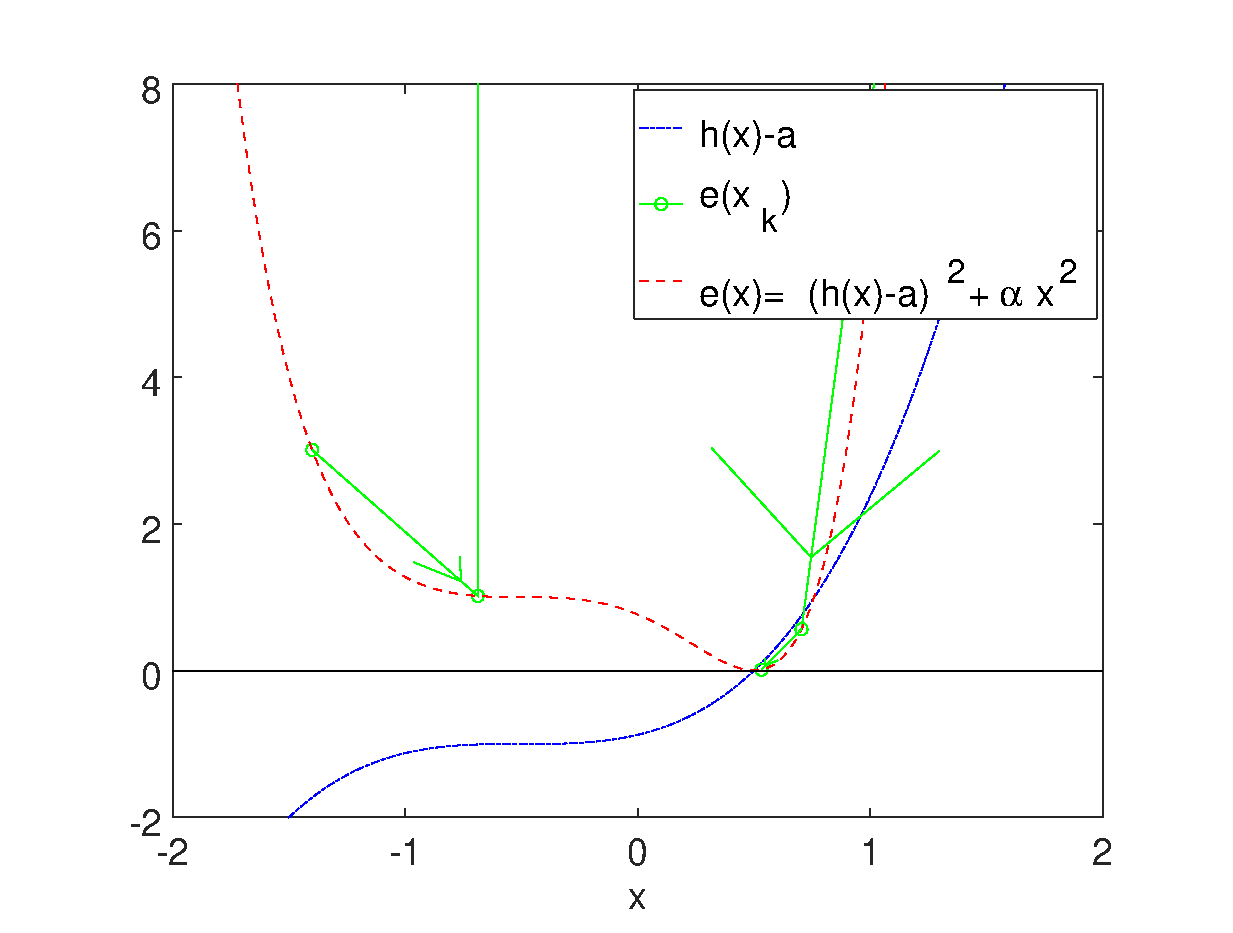
\includegraphics[width=\textwidth]{chapters/minimization-hx/mfiles/hx3_a_alphax/minimizando_hx_a_alphax_1.eps}
        \caption{Usando $h(x)=(x+0.5)^3$, $a=1$ e $\alpha=0.01$, quando as iterações divergem e logo convergem.}
        \label{fig:hx3bcasesa}
    \end{subfigure}
    ~ %add desired spacing between images, e. g. ~, \quad, \qquad, \hfill etc. 
      %(or a blank line to force the subfigure onto a new line)
    \begin{subfigure}[b]{0.49\textwidth}
        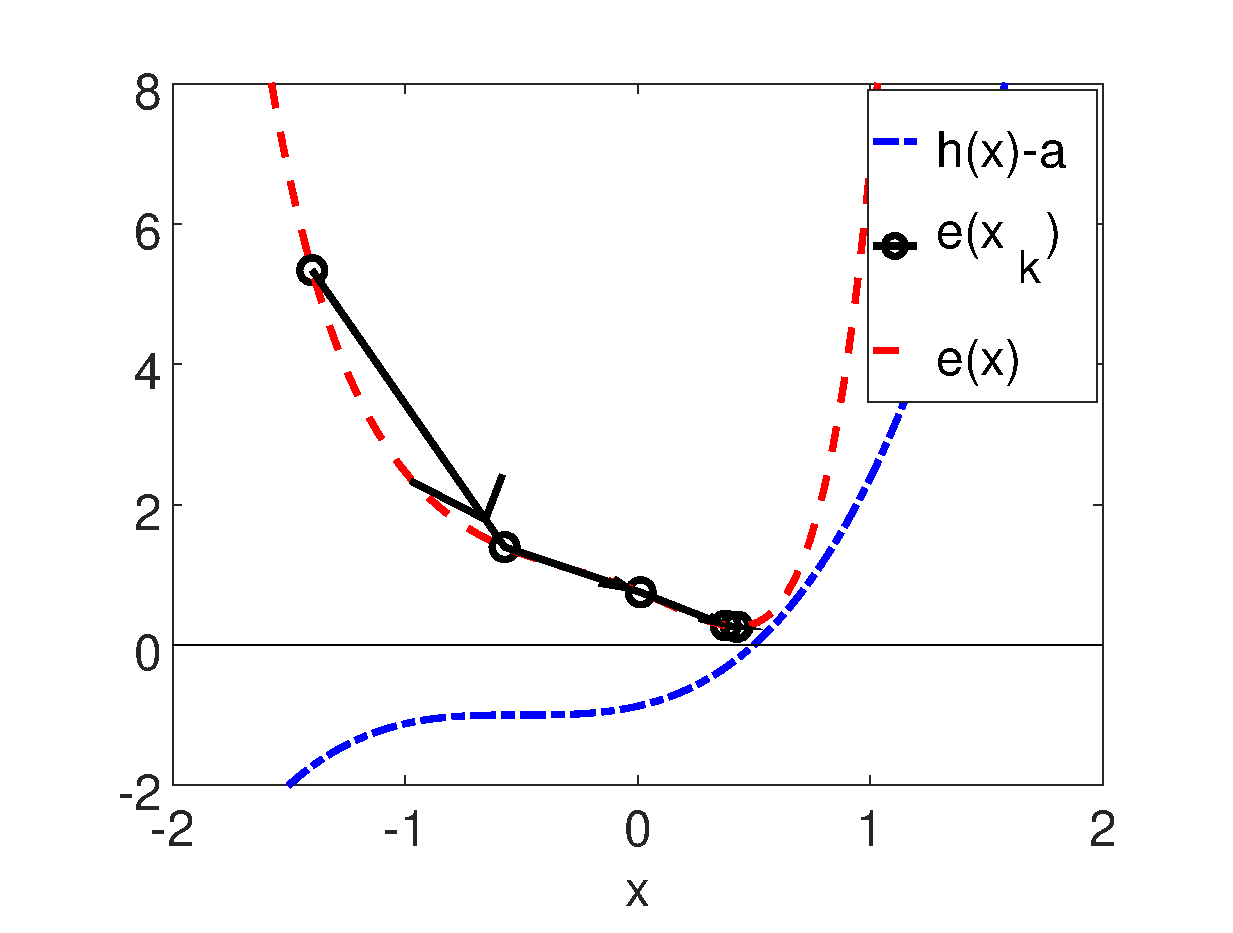
\includegraphics[width=\textwidth]{chapters/minimization-hx/mfiles/hx3_a_alphax/minimizando_hx_a_alphax_2.eps}
        \caption{Usando $h(x)=(x+0.5)^3$, $a=1$ e $\alpha=1.2$, quando as iterações convergem no mínimo global.}
        \label{fig:hx3bcasesb}
    \end{subfigure}
    \caption{Comportamento para $h(x)=(x+0.5)^3$ da equação iterativa do Teorema \ref{theo:minhxhxxbxb}.}
    \label{fig:hx3bcases}
\end{figure}

\begin{example}\label{ex:minhx3hx3xbxb4}
Conhecida uma função $h(x)=(x+0.5)^3$, o valor $a=1$ no contradomínio de $h(x)$,
o fator $\alpha=1.2$ e o ponto $b=0$,
achar o valor $x=\hat{x}$ que minimize $e(x)=||h(x)-a||^2+\alpha||x-b||^2$.
\end{example}
\begin{SolutionT}[Relativa ao Exemplo \ref{ex:minhx3hx3xbxb4}:]\label{sol:minhx3hx3xbxb4}
 A Fig. \ref{fig:hx3bcasesb} nos mostra o processo de busca de um mínimo
 de $e(x)$. A busca inicia em $x_0=-1.4$,
 todos os valores $x_{k}$ podem ser vistos na Tabela \ref{tab:hx3bcases4}. 
Neste caso, a busca iterativa indicada pela Eq. (\ref{eq:minhxhxxbxb2}) converge 
em $\hat{x}\approx x_7=+0.428757$ com $e(\hat{x})\approx 0.26$,
que é o mínimo global de $e(x)$.
\begin{comment}
; porém, este valor de $x_k$ está
um pouco distante do mínimo de $(h(x)-a)^2$, localizado em $x=+0.5$.
Novamente, isto é consequência do uso do fator 
 $\alpha>0$ e grande.
\end{comment}
\end{SolutionT}


\begin{table}[!h]
\centering
\begin{tabular}{|l|l|l|l|l|l|l|l|l|}
\hline
$k$      & 0 & 1 & 2 & 3 & 4 & 5 & 6 & 7 \\ \hline
$x_k$    & -1.40000 & -0.57219  & 0.01292  & 0.37895  & 0.42295  & 0.42797  & 0.42866  & 0.42876 \\ \hline
$e(x_k)$ &  5.34144 &  1.39364  & 0.74853  & 0.27534  & 0.26037  & 0.26015  & 0.26015  & 0.26015 \\ \hline
\end{tabular}
\caption{Resposta iterativa do Exemplo \ref{ex:minhx3hx3xbxb4}.}
\label{tab:hx3bcases4}
\end{table}


